\documentclass[a4paper,11pt]{article}
\usepackage[utf8]{inputenc}
\usepackage[a4paper,margin=0.8in]{geometry}
\usepackage{amsmath}
\usepackage{amsfonts}
\usepackage{amssymb}
\usepackage{listings}
\usepackage{xcolor}
\usepackage{graphicx}

\definecolor{slack-bg}{HTML}{FFFFFF}
\definecolor{slack-fg}{HTML}{1A1D21}
\definecolor{slack-keyword}{HTML}{36C5F0}
\definecolor{slack-string}{HTML}{2EB67D}
\definecolor{slack-comment}{HTML}{A5A5A5}
\definecolor{slack-number}{HTML}{E01E5A}

\lstset{
  backgroundcolor=\color{slack-bg},
  basicstyle=\ttfamily\footnotesize\color{slack-fg},
  keywordstyle=\color{slack-keyword},
  stringstyle=\color{slack-string},
  commentstyle=\color{slack-comment},
  numberstyle=\color{slack-number},
  frame=single,
  rulecolor=\color{slack-bg},
  framesep=8pt,
  xleftmargin=15pt,
  xrightmargin=15pt,
  showstringspaces=false,
  numbers=left,
  numbersep=10pt,
  numberstyle=\tiny\color{slack-number}
}

\title{\Huge\textbf{Documenta\c{t}ie Proiect} \\ \Large Probabilitate si Statistica}
\author{\textbf{Membri:} \\ Gheorghe Bogdan-Alexandru \\ Andrei Cristian-David \\ Sincari Sebastian-George \\ Cosor Mihail}
\date{\textbf{Ianuarie 2025}}

\begin{document}

\begingroup
\centering
\maketitle
\endgroup

\tableofcontents

\newpage

\section*{Cerinta I}
\addcontentsline{toc}{section}{Cerinta I}

\subsection*{Descrierea Problemei}

Se consideră o activitate care presupune parcurgerea secvențială a \( n \) etape. Timpul necesar finalizării etapei \( i \) de către o persoană \( A \) este o variabilă aleatoare \( T_i \sim \text{Exp}(\lambda_i) \).

După finalizarea etapei \( i \), \( A \) va trece în etapa \( i+1 \) cu probabilitatea \( \alpha_i \) sau va opri lucrul cu probabilitatea \( 1 - \alpha_i \).

Fie \( T \) timpul total petrecut de persoana \( A \) în realizarea activității respective.

\begin{lstlisting}[language=R]
set.seed(123)
n <- 100 # Nr etape
lambda <- runif(n, 0.5, 2) # Rata exp pt fiecare etapa
alpha <- runif(n-1, 0.8, 1) # Prob trecerii la urmatoarea etapa
alpha <- c(1, alpha) # Prob ca o persoana sa participe la prima etapa este 100%
nrSimulari <- 1000000 # Nr simulari


simulator <- function() {
  Ti <- rexp(n, rate = lambda)  # Timpul pentru fiecare etapa

  stop_point <- which(runif(n - 1) > alpha[-1])[1]  # Determinam momentul opririi

  # Timpul total va fi cel pana la oprire/finalul vectorului daca nu se opreste
  if (!is.na(stop_point)) {
    return(sum(Ti[1:stop_point])) 
  } else {
    return(sum(Ti))
  }
}

# Simulam 10^6
valoriT <- replicate(nrSimulari, simulator())
\end{lstlisting}
\textbf{1. Construiți un algoritm în R care simulează $10^6$ valori pentru v.a. $T$ și în \\baza acestora aproximați $E(T)$. Reprezentați grafic într-o manieră adecvată valorile \\obținute pentru $T$. Ce puteți spune despre repartiția lui $T$?}

\begin{lstlisting}[language=R]
approx_E_T <- mean(valoriT)

hist(valoriT, breaks = 100, main = "Distributia timpilor T", xlab = "T")
\end{lstlisting}

\textbf{Explicații:}

Pentru calculul aproximativ al mediei am făcut pur și simplu media valorilor rezultate în urma simulării.

Afișând în histograma valorile obținute în \texttt{valoriT} rezultă distribuția lui $T$. Se poate observa că reprezentarea grafică a timpiilor $T$ urmează o distribuție exponențială.

\begin{figure}[h!]
    \centering
    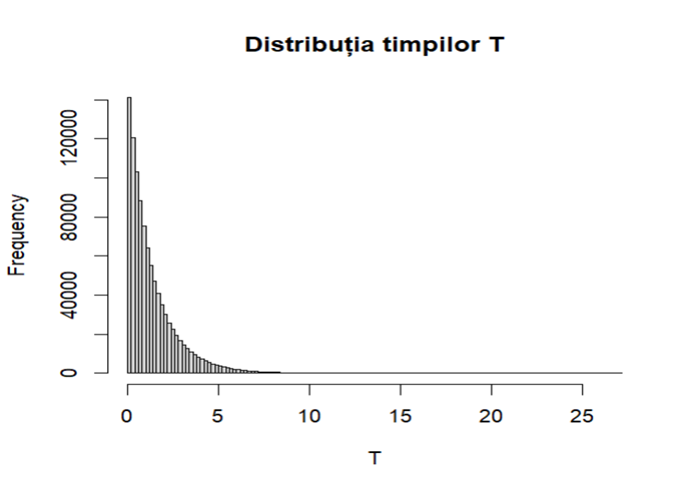
\includegraphics[width=0.56\textwidth]{./img/1.png} % Înlocuiește cu numele fișierului
    \label{fig:imaginea_ta}
\end{figure}

\newpage
\textbf{Rezultat:}
\begin{lstlisting}[language=R]
approx_E_T = 9.51113170988666
\end{lstlisting}

\textbf{2. Calculați valoarea exactă a lui $E[T]$ și comparați cu valoarea obținută prin \\simulare.}
\begin{lstlisting}[language=R]
exact_E_T <- sum(1 / \lambda * cumprod(alpha))
\end{lstlisting}

\textbf{Explicații:} 

Valoarea exactă a lui \( E[T] \) se calculează după următoarea formulă:
\[
E[T] = E[T_1] + \alpha_1 E[T_2] + \alpha_1 \alpha_2 E[T_3] + \ldots + \alpha_1 \alpha_2 \ldots \alpha_{n-1} E[T_n]
\]

Am folosit funcția \texttt{cumprod}, care returnează un vector cu produsul cumulativ. \(\alpha\) are 99 de valori deoarece există \( n-1 \) pași pentru trecerea de la o etapă la alta. Am atașat acestui vector la început valoarea 1, deoarece probabilitatea ca persoana să participe la prima etapă este 100. Apoi am înmulțit produsul cumulativ cu \( 1/\lambda \), deoarece \( X \sim \text{Exp}(\lambda) \Rightarrow E[X] = 1/\lambda \). În final, am făcut suma tuturor mediilor pe fiecare etapă, rezultând \( E[T] \).

În urma analizării rezultatului exact observăm că este foarte apropiat de rezultatul aproximativ obținut prin simulare.

\textbf{Rezultat:}
\begin{lstlisting}[language=R]
    exact_E_T = 9.51299920302413
\end{lstlisting}

\textbf{3. În baza simulărilor de la 1. aproximați probabilitatea ca persoana A să finalizeze activitatea.}
\begin{lstlisting}[language=R]
    prob_finalizare <- mean(valoriT >= sum(1 / lambda))
\end{lstlisting}
\textbf{Explicatii:} 

Am calculat probabilitatea ca o persoana sa finalizeze fiecare etapa luand ca exemplu in simularea noastra un numar de 100 de etape si o probabilitate de a trece de la o etapa la alta >=80% pentru un rezultat mai consistent.

In scrierea codului am calculat valoarea teoretica a timpului total pe care o persoana trebuie sa il petreaca in cele 100 de etape pentru a spune ca a finalizat. Astfel am calculat media unui vector de valori booleene care valoarea true corespunde rezultatului unei simulari>= valoarea timpului adica persoanele care au finalizat respectiv false pentru persoanele care nu au reusit sa finalizeze. Rezultatul este mic datorita numarului de etape, acesta ar creste o data cu micsorarea numarului de etape/ ar scadea o data cu cresterea numarului de etape. Totodata, rezultatul va scadea odata cu micsorarea marginii inferioare a valorilor probabilitatilor din alpha si invers.
\newline
\newline
\textbf{Rezultat:}
\begin{lstlisting}[language=R]
    prob_finalizare = 0.00004
\end{lstlisting}

\textbf{4. \^{I}n baza simul\u{a}rilor de la 1. aproxima\c{t}i probabilitatea ca persoana A s\u{a} finalizeze activitatea \^{i}ntr-un timp mai mic sau egal cu $\sigma$ . }

\begin{lstlisting}[language=R]
    sigma <-94
    prob_sigma<- mean(valoriT <= sigma & valoriT >= sum(1 / lambda))
\end{lstlisting}
\textbf{Explicatii:}

Ne-am folosit de modalitatea de rezolvare a exercitiului anterior, astfel am folosit un vector de valori booleene care verifica 2 conditii <= sigma si >= valoarea timpului total, apoi am facut media si ne-a rezultat valoarea probabilitatii ca o persoana sa finalizeze intr-un timp mai mic decat sigma. Este normal ca valoarea acestei probabilitati sa fie mai mica sau egala cu valoarea probabilitatii de a finaliza.
\newline
\newline
\textbf{Rezultat:}
\begin{lstlisting}[language=R]
    prob_sigma = 0.000007
\end{lstlisting}

\textbf{5. \^{I}n baza simul\u{a}rilor de la 1. determina\c{t}i timpul minim și respectiv timpul maxim \^{i}n care persoana A finalizeaz\u{a} activitatea și reprezenta\c{t}i grafic timpii de finalizare a activit\u{a}\c{t}ii din fiecare simulare. Ce puteți spune despre repartiția acestor timpi de finalizare a activit\u{a}\c{t}ii?}
\begin{lstlisting}[language=R]
    timpMin <- min(valoriT[valoriT >= sum(1 / lambda)] )
    timpMax <- max(valoriT[valoriT >= sum(1 / lambda)] )
    cat("Timpul minim:", timpMin, "Timpul maxim:", timpMax, "\n")

    hist(valoriT[valoriT >= sum(1 / lambda)], breaks=50,
                main="Distributia timpilor de finalizare", 
                xlab="Timpul de finalizare (T)", ylab="Frecventa", 
                col="lightblue", border="black")
\end{lstlisting}

\textbf{Explicatii:}

Am considerat variabilele \texttt{timpMin} și \texttt{timpMax} pentru valorile minime și maxime ale timpilor persoanelor care au finalizat evenimentul. Am folosit funcția \texttt{min} pentru minim și, ca parametru, am dat lista de timpi simulați, filtrată de valorile mai mari decât media timpului total. Am folosit din nou, pentru reprezentarea grafică, o histogramă, deoarece aceasta ajută la identificarea repartiției. Două observații sunt faptul că numărul de persoane care au reușit să finalizeze evenimentul este foarte mic în comparație cu numărul de simulări și că se observă că repartiția este uniformă, deoarece pentru alegerea valorilor random am folosit \texttt{runif}.
\begin{figure}[h!]
    \centering
    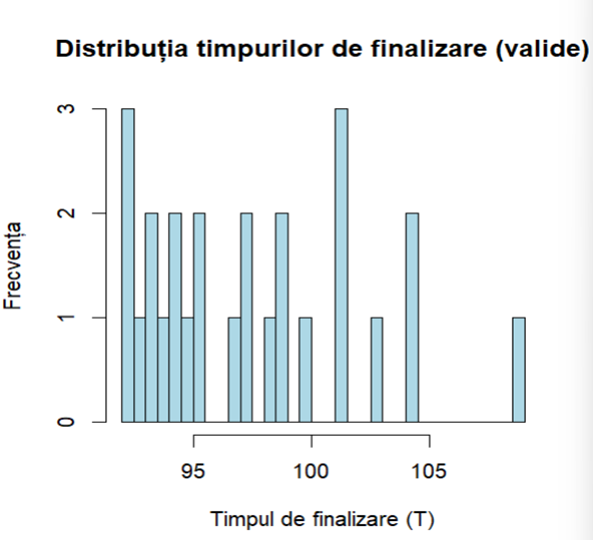
\includegraphics[width=0.56\textwidth]{./img/2.png} % Înlocuiește cu numele fișierului
    \label{fig:imaginea_ta_2}
\end{figure}

\textbf{Rezultat:}
\begin{lstlisting}[language=R]
    timpMax = 108.54443085275
    timpMin = 92.0171680316328
\end{lstlisting}

\textbf{6. \^{I}n baza simul\u{a}rilor de la 1. aproxima\c{t}i probabilitatea ca persoana A s\u{a} se opreasc\u{a} din lucru \^{i}nainte de etapa k , unde 1$<$k$\leq$n . Reprezenta\c{t}i grafic probabilit\u{a}\c{t}ile ob\c{t}inute \^{i}ntr-o manier\u{a} corespunz\u{a}toare. Ce pute\c{t}i spune despre reparti\c{t}ia probabilit\u{a}\c{t}ilor ob\c{t}inute?}

\begin{lstlisting}[language=R]
    k <- 5
    PStopK <- mean(sapply(valoriT, function(x) {
    if(x<=sum(1/lambda[1:k-1]))
        return (TRUE)
    else
        return(FALSE)
    }))
\end{lstlisting}

\textbf{Explicatii:}

Am creat o variabilă numită \texttt{PstopK} care primește probabilitatea ca persoana A să se oprească din lucru înainte de etapa k. Pentru această probabilitate am aplicat ca parametru unei funcții fiecare valoare simulată. Funcția returnează TRUE dacă timpul este mai mic decât media timpului total până la pasul k-1 (adică poate face maxim k-1 pași), și FALSE altfel. Variabila primește media valorilor din lista booleană.

\textbf{Rezultat:}
\begin{lstlisting}[language=R]
    PstopK = 0.284293  pentru k=5
    PstopK = 0.51482 pentru k=10
    PstopK = 0.991332 pentru k=50
\end{lstlisting}

\begin{lstlisting}[language=R]
    calculate_PStopBeforeK <- function(valoriT, lambda, alpha, n) {
    # Calculam timpii cumulativi pentru fiecare etapa
    cumulative_times <- cumsum(1 / lambda)
    
    # Calculam probabilitatile pentru fiecare k
    PStopBeforeK <- sapply(2:n, function(k) {
        mean(valoriT <= cumulative_times[k - 1])  
                # Probabilitatea de oprire inainte de etapa k
    })
    
    return(PStopBeforeK)
    }
    PStopBeforeK <- calculate_PStopBeforeK(valoriT, lambda, alpha, n)

    barplot(PStopBeforeK, names.arg = 2:n, col = "lightblue",
            main = "Probabilitatile de oprire inainte de etapa k",
            xlab = "Etapa k", ylab = "Probabilitatea de oprire",
            xlim = c(1, n), ylim = c(0, 1))

    
\end{lstlisting}

\begin{figure}[h!]
    \centering
    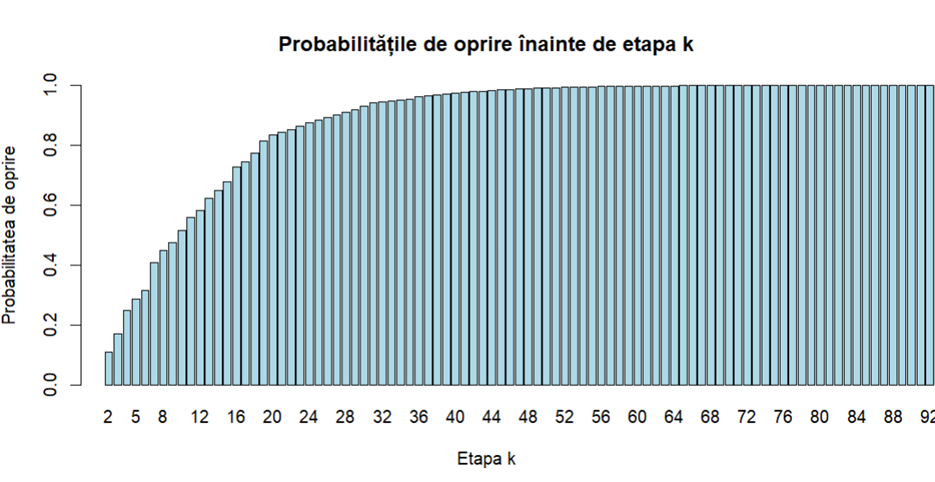
\includegraphics[width=0.8\textwidth]{./img/3.png} % Înlocuiește cu numele fișierului
    \label{fig:imaginea_ta_3}
\end{figure}
\newpage
\textbf{Observații:}

Se poate observa că o persoană, cu cât ajunge mai departe în etape, cu atât are șanse mai mari să finalizeze evenimentul, iar în etapele inițiale șansele sunt foarte mici. Aceste observații sunt date datorită pantei abrupte în faza inițială, respectiv panta lină de la final.

\newpage

\section*{Cerinta II}
\addcontentsline{toc}{section}{Cerinta II}

\subsection*{Mesaj pentru Sebi: (Pula n-are scoala ca sta sub banca)}

\newpage

\section*{Cerinta III}
\addcontentsline{toc}{section}{Cerinta III}

\subsection*{Descrierea Problemei}
\addcontentsline{toc}{subsection}{Descrierea Problemei}

Scopul acestui proiect este de a construi o aplica\c{t}ie web interactiv\u{a} folosind framework-ul \textbf{Shiny} din \textbf{R}, pentru a reprezenta grafic func\c{t}iile de reparti\c{t}ie (CDF) ale unor variabile aleatoare definite conform cerin\c{t}ei din enun\c{t}. Aplica\c{t}ia permite vizualizarea CDF-urilor pentru distribu\c{t}ii normale, exponen\c{t}iale, binomiale, Poisson.

\subsection*{Aspecte Teoretice}
\addcontentsline{toc}{subsection}{Aspecte Teoretice}
Pentru dezvoltarea aplica\c{t}iei, am utilizat urm\u{a}toarele aspecte teoretice importante:

\begin{itemize}
  \item \textbf{Distribu\c{t}ia Normal\u{a}}: Este definit\u{a} ca o variabil\u{a} aleatoare continu\u{a} $X \sim N(\mu, \sigma^2)$, unde $\mu$ reprezint\u{a} media, iar $\sigma^2$ varian\c{t}a.
  \newline
  Formula funcției de repartiție cumulativă:
  \[
  F(x) = P(X \leq x) = \int_{-\infty}^{x} \frac{1}{\sqrt{2\pi \sigma^2}} e^{-\frac{(t - \mu)^2}{2\sigma^2}} \, dt
  \]

  \item \textbf{Distribu\c{t}ia Exponen\c{t}ial\u{a}}: O variabil\u{a} aleatoare $X \sim \text{Exp}(\lambda)$ este folosit\u{a} pentru modelarea timpilor de a\c{s}teptare între evenimente.
  \newline
  Formula funcției de repartiție cumulativă:
  \[
  F(x) = P(X \leq x) = 
  \begin{cases}
  1 - e^{-\lambda x}, & \text{pentru } x \geq 0 \\
  0, & \text{pentru } x < 0
  \end{cases}
  \]

  \item \textbf{Distribu\c{t}ia Poisson}: Reprezint\u{a} num\u{a}rul de evenimente într-un interval fix de timp \c{s}i este notat\u{a} $X \sim \text{Poisson}(\lambda)$.
  \newline
  Formula funcției de repartiție cumulativă:
  \[
  F(x) = P(X \leq x) = \sum_{k=0}^{\lfloor x \rfloor} \frac{\lambda^k e^{-\lambda}}{k!}
  \]

  \item \textbf{Distribu\c{t}ia Binomial\u{a}}: Este definit\u{a} de parametrii $n$ \c{s}i $p$ \c{s}i descrie num\u{a}rul de succese în $n$ experimente independente.
  \newline
  Formula funcției de repartiție cumulativă:
  \[
  F(x) = P(X \leq x) = \sum_{k=0}^{\lfloor x \rfloor} \binom{n}{k} p^k (1 - p)^{n - k}
  \]
\end{itemize}

\newpage

\subsection*{Reprezent\u{a}ri Grafice}
\addcontentsline{toc}{subsection}{Reprezent\u{a}ri Grafice}

Aplica\c{t}ia ofer\u{a} reprezent\u{a}ri grafice ale func\c{t}iilor de reparti\c{t}ie pentru fiecare dintre variabilele aleatoare definite în cerin\c{t}e. În cele ce urmeaz\u{a}, vom ilustra c\u{a}teva capturi de ecran din aplica\c{t}ie.

\begin{figure}[h!]
  \centering
  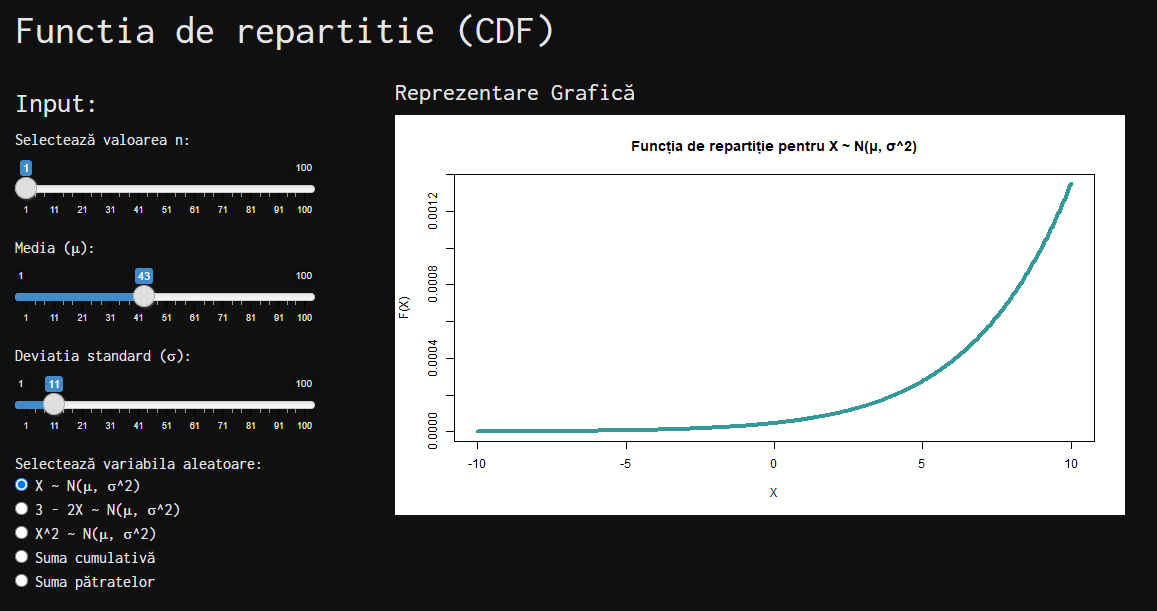
\includegraphics[width=0.8\textwidth]{./img/4.png}
  \label{fig:imaginea_ta_3}
\end{figure}

\begin{figure}[h!]
  \centering
  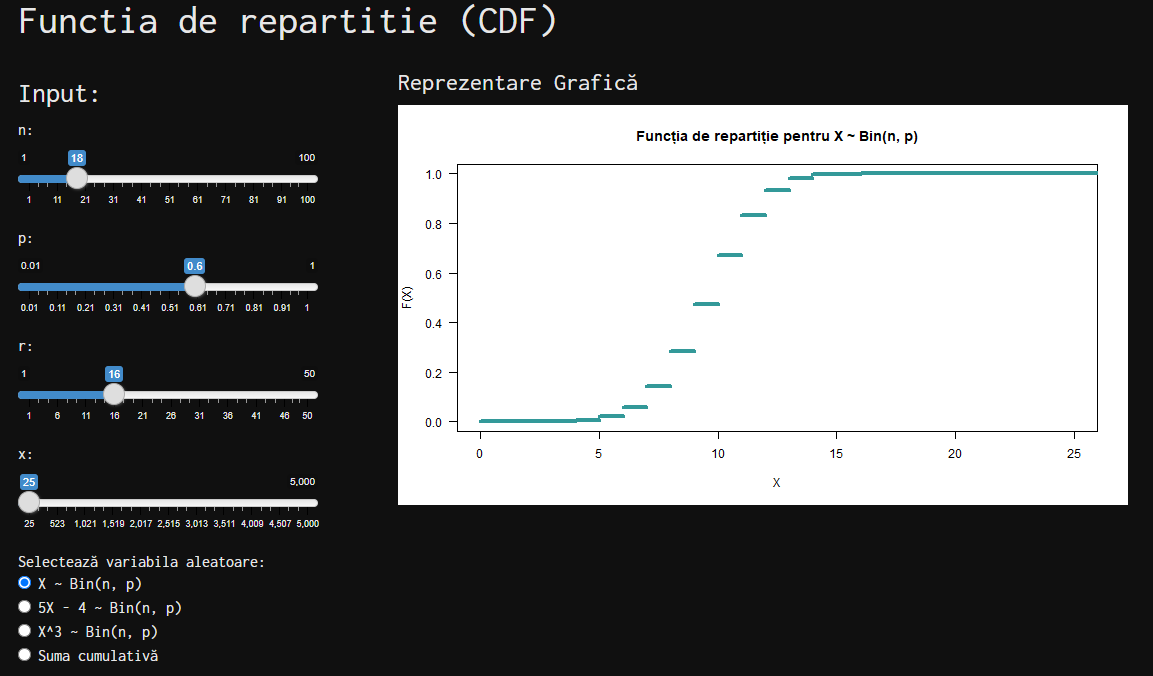
\includegraphics[width=0.8\textwidth]{./img/5.png}
  \label{fig:imaginea_ta_3}
\end{figure}

\subsection*{Pachete Software Folosite}
\addcontentsline{toc}{subsection}{Pachete Software Folosite}

Am folosit urm\u{a}toarele pachete software pentru implementarea proiectului:

\begin{itemize}
    \item \textbf{shiny}: Crearea aplica\c{t}iei interactive.
    \item \textbf{bslib}: Personalizarea interfe\c{t}ei grafice a aplica\c{t}iei folosind teme Bootstrap.
    \item \textbf{graphics}: Generarea reprezent\u{a}rilor grafice ale func\c{t}iilor de reparti\c{t}ie.
\end{itemize}

\newpage

\subsection*{Codul Aplica\c{t}iei}
\addcontentsline{toc}{subsection}{Codul Aplica\c{t}iei}

Codul aplicației a fost structurat în mai multe fișiere pentru a asigura o separare clară a logicii și o reutilizare ușoară a funcțiilor. Această abordare are ca scop evitarea redundanței și îmbunătățirea clarității codului, permițând adăugarea sau modificarea distribuțiilor fără a afecta structura generală a aplicației.

\subsubsection*{app.R}
\addcontentsline{toc}{subsubsection}{app.R}

Fișierul principal \textbf{app.R} conține doar partea de inițializare a aplicației Shiny, inclusiv încărcarea fișierelor \texttt{ui.R}, \texttt{utils.R} și \texttt{server/server.R}. Aceasta facilitează gestionarea centralizată a componentelor aplicației.
Fiecare distribuție are propriile fișiere în directorul \texttt{server}, în care sunt definite logicile de generare a graficelor corespunzătoare.

\begin{lstlisting}[language=R, basicstyle=\ttfamily\footnotesize, keywordstyle=\color{blue}\bfseries, commentstyle=\color{green!60!black}, stringstyle=\color{orange}]
library(shiny)
library(bslib)

source("utils.R")
source("ui.R")
source("server/server.R")

shinyApp(ui = ui, server = server)
\end{lstlisting}

\subsubsection*{ui.R}
\addcontentsline{toc}{subsubsection}{ui.R}

Interfața utilizatorului este creată folosind funcția \texttt{fluidPage}, care organizează interfața pe tab-uri, câte unul pentru fiecare distribuție (normală, exponențială, binomială, Poisson). Fiecare tab este generat folosind funcția personalizată \texttt{create\_tab}, care asociază un input specific distribuției respective și o zonă de afișare a graficului.

\begin{lstlisting}[language=R]
  source("server/server.R")

  create_tab <- function(tab_title, title, distribution) {
    tabPanel(
      tab_title,
      div(
        class = "container",
        h1(title),
        div(
          class = "row",
          div(
            class = "col-4",
            tags$h3("Input:"),
            switch(
              distribution,
              BINOMIALA = create_binom_slider(),
              NORMALA_STANDARD = create_std_normal_slider(),
              NORMALA = create_normal_slider(),
              EXPONENTIALA = create_exponential_slider(),
              POISSON = create_pois_slider()
            )
          ),
          div(
            class = "col-8",
            h4("Reprezentare Grafica"),
            get_output_distribution(distribution)
          )
        )
      )
    )
  }
  
  ui <- fluidPage(
    theme = bs_theme(
      version = 4, 
      bg = "#101010", 
      fg = "#FFF", 
      primary = "#E69F00", 
      base_font = font_google("Inconsolata")
    ),
    navbarPage(
      "CDF",
      create_tab(
        "Normala Standard",
        "Functia de repartitie (CDF)",
        NORMALA_STANDARD
      ),
      create_tab(
        "Normala",
        "Functia de repartitie (CDF)",
        NORMALA
      ),
      create_tab(
        "Exponentiala",
        "Functia de repartitie (CDF)",
        EXPONENTIALA
      ),
      create_tab(
        "Binomiala",
        "Functia de repartitie (CDF)",
        BINOMIALA
      ),
      create_tab(
        "Poisson",
        "Functia de repartitie (CDF)",
        POISSON
      )
    )
  )  
\end{lstlisting}

\subsubsection*{server.R}
\addcontentsline{toc}{subsubsection}{server.R}

Acesta este punctul central al logicii serverului. Codul serverului include apeluri către fișierele individuale ale fiecărei distribuții, cum ar fi \texttt{std\_normal.R}, \texttt{normal.R}, \texttt{binom.R} etc. Acest lucru permite fiecărei distribuții să fie tratată separat și modular, facilitând adăugarea sau modificarea distribuțiilor fără a afecta alte componente.

\begin{lstlisting}[language=R]
  source("server/std_normal.R")
  source("server/normal.R")
  source("server/exponential.R")
  source("server/binom.R")
  source("server/poisson.R")
  
  server <- function(input, output, session) {
    std_normal_server(input, output, session)
    normal_server(input, output, session)
    exponential_server(input, output, session)
    binom_server(input, output, session)
    pois_server(input, output, session)
  }
  
\end{lstlisting}

\subsubsection*{utils.R}
\addcontentsline{toc}{subsubsection}{utils.R}

Acest fișier conține definiții comune, cum ar fi identificatorii fiecărei distribuții și funcția \texttt{get\_output\_distribution}, care returnează componenta grafică potrivită pentru distribuția selectată. Aceasta contribuie la eliminarea duplicării codului și la centralizarea logicii de redirecționare a graficelor.

\begin{lstlisting}[language=R]
  NORMALA_STANDARD <- "NORMALA_STANDARD"
  NORMALA <- "NORMALA"
  EXPONENTIALA <- "EXPONENTIALA"
  BINOMIALA <- "BINOMIALA"
  POISSON <- "POISSON"
  
  get_output_distribution <- function(distribution) {
    switch(
      distribution,
      NORMALA_STANDARD = plotOutput("std_normal_plot"),
      NORMALA = plotOutput("normal_plot"),
      EXPONENTIALA = plotOutput("exponential_plot"),
      BINOMIALA = plotOutput("binom_plot"),
      POISSON = plotOutput("pois_plot")
    )
  }
\end{lstlisting}

\subsubsection*{normals.R}
\addcontentsline{toc}{subsubsection}{normals.R}

\paragraph{Generarea graficelor:}  
Codul pentru reprezentarea grafică este similar pentru toate distribuțiile, însă exemplificarea este prezentată doar pentru distribuția normală în fișierul \texttt{normals.R}.  
Fiecare grafic este generat pe baza parametrilor selectați de utilizator (cum ar fi media \(\mu\) și deviația standard \(\sigma\)) și utilizează funcția corespunzătoare de calcul al funcției de repartitie cumulativă. Iată principalele tipuri de grafice generate:

- **Graficul funcției de repartitie cumulativă (CDF)**: Este reprezentată funcția \( F(x) = P(X \leq x) \), calculată cu funcția R corespunzătoare fiecărei distribuții (de exemplu, \texttt{pnorm} pentru distribuția normală).
  
- **Transformări ale variabilelor**: De exemplu, pentru \( 3 - 2X \) sau \( X^2 \), transformările sunt aplicate asupra datelor înainte de a calcula și reprezenta \( F(x) \).
  
- **Sumă cumulativă**: Pentru a reprezenta suma cumulativă \( \sum X_i \) sau \( \sum X_i^2 \), se utilizează funcția \texttt{cumsum} din R, iar graficul este construit prin afișarea acestor sume pentru fiecare \( n \).

\begin{lstlisting}[language=R]
  create_normal_slider <- function() {
    tagList(
      sliderInput(
        inputId = "normal_n",
        label = "Selecteaza valoarea n:",
        min = 1,
        max = 100,
        value = 10,
        step = 1
      ),
      sliderInput(
        inputId = "normal_mu",
        label = "Media (\u03BC):",
        min = 1,
        max = 100,
        value = 10,
        step = 1
      ),
      sliderInput(
        inputId = "normal_sigma",
        label = "Deviatia standard (\u03C3):",
        min = 1,
        max = 100,
        value = 10,
        step = 1
      ),
      radioButtons(
        inputId = "normal_var",
        label = "Selecteaza variabila aleatoare:",
        choices = list(
          "X ~ N(\u03BC, \u03C3^2)" = "var1",
          "3 - 2X ~ N(\u03BC, \u03C3^2)" = "var2",
          "X^2 ~ N(\u03BC, \u03C3^2)" = "var3",
          "Suma cumulativa" = "var4",
          "Suma patratelor" = "var5"
        ),
        selected = "var1"
      )
    )
  }
  
  normal_server <- function(input, output, session) {
    output$normal_plot <- renderPlot({
      var <- input$normal_var
      
      if (var == "var1") {
        x <- seq(-10, 10, length.out = 500)
        cdf_values <- pnorm(x, mean = input$normal_mu, sd = input$normal_sigma)
        plot(
          x, cdf_values,
          type = "l",
          lwd = 4,
          col = "#339999",
          xlab = "X",
          ylab = "F(X)",
          main = "Functia de repartitie pentru X ~ N(\u03BC, \u03C3^2)"
        )
      } else if (var == "var2") {
        x <- seq(-10, 10, length.out = 500)
        transformed_x <- 3 - 2 * x
        cdf_values <- pnorm(transformed_x, mean = input$normal_mu, sd = input$normal_sigma)
        plot(
          x, cdf_values,
          type = "l",
          lwd = 4,
          col = "#FF6666",
          xlab = "3 - 2X",
          ylab = "F(3 - 2X)",
          main = "Functia de repartitie pentru 3 - 2X ~ N(\u03BC, \u03C3^2)"
        )
      } else if (var == "var3") {
        x <- seq(-10, 10, length.out = 500)
        transformed_x <- x^2
        cdf_values <- pnorm(transformed_x, mean = input$normal_mu, sd = input$normal_sigma)
        plot(
          x, cdf_values,
          type = "l",
          lwd = 4,
          col = "#3399FF",
          xlab = "X^2",
          ylab = "F(X^2)",
          main = "Functia de repartitie pentru X^2 ~ N(\u03BC, \u03C3^2)"
        )
      } else if (var == "var4") {
        n <- input$normal_n
        X <- rnorm(n, mean = input$normal_mu, sd = input$normal_sigma)
        S_n <- cumsum(X)
        plot(
          1:n, S_n,
          type = "l",
          lwd = 2,
          col = "#FF9900",
          xlab = "n",
          ylab = "\u2211 X_i",
          main = "Suma cumulativa a variabilelor aleatoare X_i"
        )
      } else if (var == "var5") {
        n <- input$normal_n
        X <- rnorm(n, mean = input$normal_mu, sd = input$normal_sigma)
        S_n2 <- cumsum(X^2)
        plot(
          1:n, S_n2,
          type = "l",
          lwd = 2,
          col = "#33CC33",
          xlab = "n",
          ylab = "\u2211 X_i^2",
          main = "Suma cumulativa a patratelor variabilelor X_i"
        )
      }
    })
  }
\end{lstlisting}

\subsection*{Dificult\u{a}\c{t}i Întâmpinate}
\addcontentsline{toc}{subsection}{Dificult\u{a}\c{t}i Întâmpinate}

Dezvoltarea aplicației a implicat rezolvarea unor provocări tehnice importante legate de gestionarea parametrilor și a reprezentărilor grafice pentru fiecare distribuție. Principalele dificultăți întâmpinate sunt:

\begin{itemize}
    \item \textbf{Ajustarea automată a parametrilor pentru fiecare distribuție:}  
    Fiecare distribuție are un set unic de parametri care trebuie adaptați corect pentru a asigura o reprezentare grafică precisă a funcției de repartitie cumulativă (CDF). De exemplu, distribuția normală implică media \(\mu\) și deviația standard \(\sigma\), în timp ce distribuția binomială depinde de numărul de experimente \(n\) și probabilitatea de succes \(p\). Provocarea a fost legată de crearea unui sistem flexibil în care utilizatorul să poată modifica rapid parametrii în interfață, iar graficele să se actualizeze automat în funcție de aceștia. Această problemă a fost rezolvată prin implementarea unor funcții modulare (de exemplu, \texttt{create\_normal\_slider()} și \texttt{create\_binom\_slider()}) care generează dinamic controale de input specifice fiecărei distribuții.
\end{itemize}

\subsection*{Probleme Deschise}
\addcontentsline{toc}{subsection}{Probleme Deschise}

Deși aplicația funcționează corespunzător și oferă o interfață interactivă pentru vizualizarea funcțiilor de repartitie cumulativă, există câteva direcții de dezvoltare viitoare și probleme deschise:

\begin{itemize}
    \item \textbf{Posibilitatea extinderii aplicației pentru a suporta și alte distribuții:}  
    Momentan, aplicația suportă distribuțiile normală, exponențială, binomială și Poisson. Cu toate acestea, există o varietate de alte distribuții utile în statistică, cum ar fi distribuțiile Bernoulli, binomiale sau geometrice, care ar putea fi integrate cu ușurință în structura modulară a aplicației. O extindere în această direcție ar implica adăugarea fișierelor corespunzătoare în directorul \texttt{server} și crearea funcțiilor de input specifice fiecărei noi distribuții.
\end{itemize}

\subsection*{Concluzii}
\addcontentsline{toc}{subsection}{Concluzii}

Funcționalitățile existente permit utilizatorilor să vizualizeze funcțiile de repartitie ale variabilelor normale, exponențiale, binomiale și Poisson, dar structura modulară face posibilă integrarea rapidă a altor distribuții. De asemenea, prin intermediul graficelor dinamice, utilizatorii pot explora nu doar distribuțiile de bază, ci și diverse transformări ale variabilelor aleatoare, cum ar fi transformări liniare și sume cumulative.

\end{document}